Find the equation of the circle with radius 5 whose centre lies on $x$-axis and passes through the point $\brak{2,3}$.

\textbf{Solution :}
\begin{table}[H]
    \centering
        \begin{tabular}{|c|c|c|}
    \hline
         \textbf{Input parameters}& \textbf{Description}&\textbf{Value} \\
         \hline
         $r$ & Radius&$5$ \\
        \hline
        $\vec{O}$ & Center&$x\vec{e_1}$ \\
        \hline
       $\vec{A}$&Point &$\myvec{2\\3}$ \\
       \hline
    \end{tabular}

        \caption{Table of input parameters}
    \label{tab:11.11.1.13}
\end{table}
The general formula of the circle is
\begin{align}
\norm{\vec{x}}^2 + 2\vec{u}^{\top}\vec{x}+f&=0\\
	where,   \vec{u}&=-x\vec{e_1}\\
	f&=\norm{\vec{O}}-r^2\\
f&=x-r^2\\
\norm{\vec{A}}^2 + 2\vec{u}^{\top}\vec{A}+f&=0\\
13-4x+x-r^2&=0\\
or,x&=-4\\
or,f&=-29
\end{align}
Therefore the equations of the circle are
\begin{align}
   \norm{\vec{x}}^2 - 2\myvec{-4&0}\vec{x}-29&=0\\
\end{align}    
\begin{figure}[H]
    \centering
	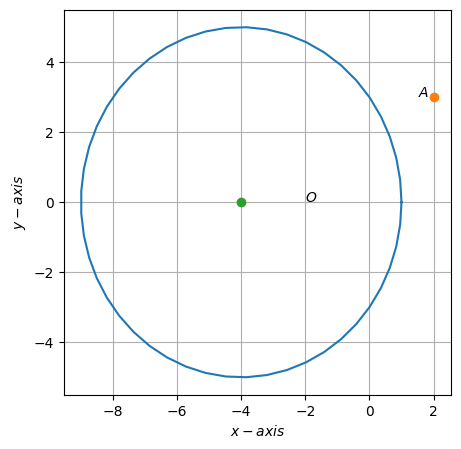
\includegraphics[width=\columnwidth]{chapters/11/11/1/13/fig/11.11.1.13.png}
    \caption{}
    \label{fig:11.11.1.13}
\end{figure}


